\documentclass[a4paper,11pt]{article}

%% Language and font encodings
\usepackage[english]{babel}
\usepackage[utf8x]{inputenc}
\usepackage[T1]{fontenc}
\usepackage{subcaption}

%% Sets page size and margins
\usepackage[a4paper,top=3cm,bottom=2cm,left=3cm,right=3cm,marginparwidth=2cm]{geometry}

%% Useful packages
\usepackage{amsmath}
\usepackage{graphicx}
\usepackage[colorinlistoftodos]{todonotes}
\usepackage[colorlinks=true, allcolors=blue]{hyperref}




\begin{document}

\vspace*{13mm}
\begin{center}
\rule[0.5ex]{\linewidth}{2pt}\vspace*{-\baselineskip}\vspace*{3.2pt}
\rule[0.5ex]{\linewidth}{1pt}\\[\baselineskip]
{\Huge Robust Augmented Reality using RGB-D SLAM}\\[4mm]

\rule[0.5ex]{\linewidth}{1pt}\vspace*{-\baselineskip}\vspace{3.2pt}
\rule[0.5ex]{\linewidth}{2pt}\\
\vspace{6.5mm}
{\large By}\\
\vspace{6.5mm}
{\large\textsc{Ze Zhang}}\\
\vspace{11mm}

\includegraphics[scale=0.6]{bristolcrest_colour}\\
\vspace{6mm}
{\large Department of Engineering Mathematics\\
\textsc{University of Bristol}}\\
\vspace{11mm}
\begin{minipage}{10cm}

\end{minipage}\\
\vspace{9mm}
{\large\textsc{31 March 2017}}
\vspace{12mm}
\end{center}

\newpage
\section{Aims and Objectives}
\subsection{Aims}
This project will study how to develop a robust Augmented Reality (AR) system based on RGB-D SLAM system. This AR system will use the accurate 3D model which is generated by SLAM system, so it is more robust and accurate than most other AR system. 
\subsection{Objectives}
\begin{itemize}
\item Study RGB-D SLAM system.
\item Connect new RGB-D sensor with SLAM system.
\item Using SLAM system to contrast 3D model.
\item Using AR software to create virtual character.
\item Apply AR system in google map if time permits.
\end{itemize}


\section{Motivation}
AR and VR are two hot concept today, prevalent people also know them as VR film and AR game. I know AR because of the famous mobile game pokemon go which is showed in figure 1a. Then I find another AR app called SekaiCamera which is developed by Japanese company Tonchidot in figure 1b. It can add comments on object which is captured by your phone camera. I think AR is more useful than VR because it adds information on real scene instead of create a new scene. However, pokemon go and SekaiCamera are simple AR systems which only use 2D image and GPS. I want to develop a more robust AR system based on accurate 3D model which is provided by RGB-D SLAM system.

\begin{figure}[!htp]
		\centering
		\begin{subfigure}{.5\textwidth}
			\centering
			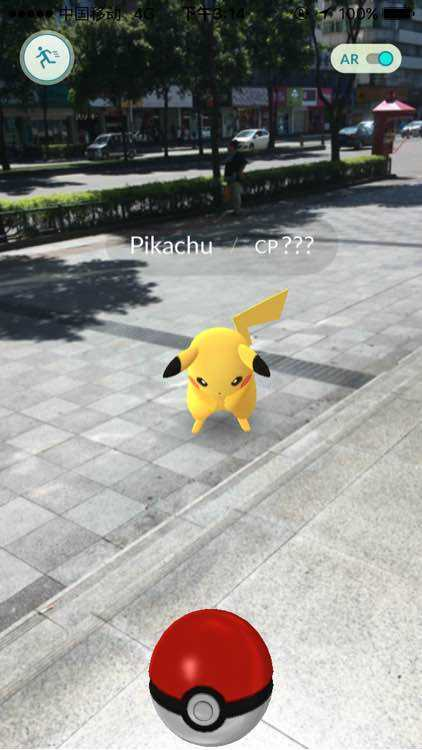
\includegraphics[width=0.7\linewidth]{1.jpg}
			\caption{pokemon go}
		
		\end{subfigure}%
		\begin{subfigure}{.5\textwidth}
			\centering
			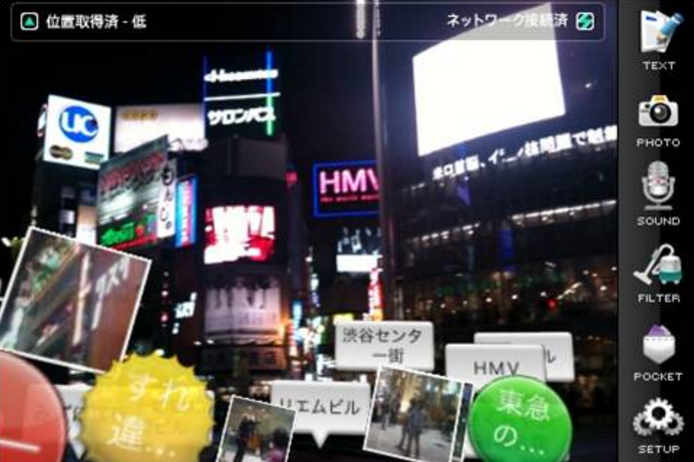
\includegraphics[width=1.2\linewidth]{2.png}
			\caption{SekaiCamera}
			
		\end{subfigure}
		\caption{AR system}
		\label{fig:fig1}
	\end{figure}


\newpage
\section{Literature Review}
\subsection{Visual based SLAM}
Simultaneous Localisation and Mapping (SLAM) is a process that a mobile robot builds a complete map of an unknown environment and note its own location in this map. The solution of this problem is an important sign for mobile robotics which means the mobile robot is truly autonomous. To solve this problem, a lot of approaches have been developed. The most popular one is Kalman filter based approach. This approach is popular because it directly provides recursive solutions to the navigation problem and the uncertainty of vehicle and map landmark locations based on statistical motion model of vehicle and observation model of landmarks \cite{938381}. Details are shown in figure 2.

\begin{figure}[!htp]


\centering
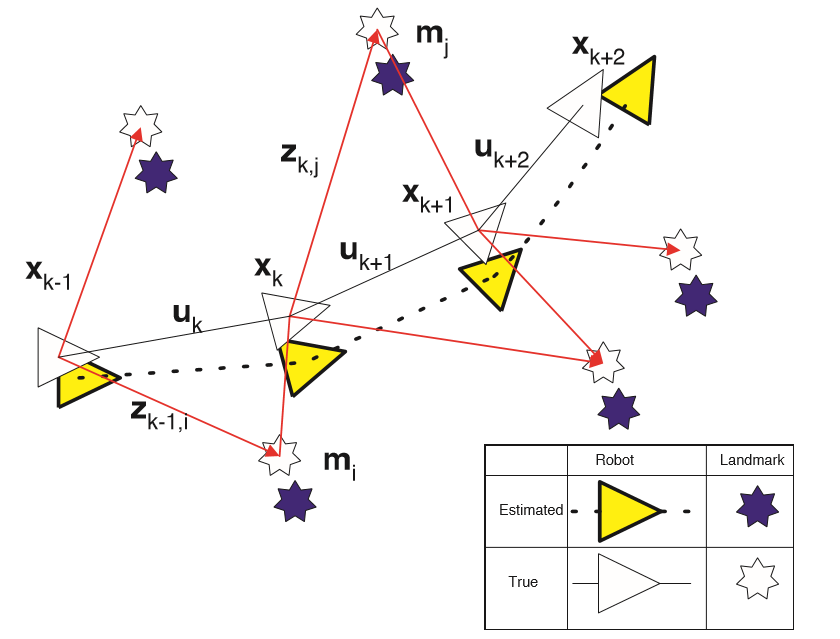
\includegraphics[width=1\textwidth]{3.png}
\caption{\label{fig:frog}Details of SLAM problem}
\end{figure}
In this figure, xk is the state vector describing the location and orientation of the vehicle, uk is the control vector, vehicle move from xk-1 to xk in time k, mi is the location of landmark, zkj is an observation model of landmark mj viewing from xk. Our goal is obtaining the probability distribution of the relative positions of vehicle and landmarks which means the map \cite{1638022}:
\begin{equation}
P(x_k,m | Z_{0:k}, U_{0:k}, x_0)
\end{equation}
For calculating this probability distribution, motion model and observation model are necessary, which are described in following form respectively.
\begin{equation}
P(x_k | x_{k-1}, u_k)
\end{equation}
\begin{equation}
P(z_k | x_k, m)
\end{equation}

With motion model and observation model, a recursive process can be calculated, which are prediction and correction describing in following form respectively.
\begin{equation}
P(x_k,m | Z_{0:k-1}, U_{0:k}, x_0)=\int P(x_k | x_{k-1}, u_k)P(x_{k-1},m | Z_{0:k-1}, U_{0:k-1}, x_0)dx_{k-1}
\end{equation}
\begin{equation}
P(x_k,m | Z_{0:k}, U_{0:k}, x_0)=\frac{P(z_k | x_k, m)P(x_k,m | Z_{0:k-1}, U_{0:k}, x_0)}{P(z_k | Z_{0:k-1}, U_{0:k})}
\end{equation}

After this recursive process, a map can be built by landmarks. In addition, the location of vehicle can be determined by the observation results.

\subsection{RGB-D SLAM}


\subsection{Augmented reality using RGB-D slam}


\section{Risk register}


\begin{table}[!htp]
\caption{\label{tab:widgets}Risks}
\centering
\begin{tabular}{ | p{0.5cm}| p{4.5cm}|p{4cm} | p{1.9cm}| p{1.2cm} | p{1.2cm} | }

\hline
 &\textbf{Risks}&\textbf{Mitigation}&\textbf{Likelihood}&\textbf{Impact}&\textbf{Score}\\ 
\hline
\textbf{1}&Can not understand RGB-D SLAM system&Ask research assistant immediately when some code is difficult to understand&1&3&3\\ 
\hline
\textbf{2}&Late arrive of RGB-D sensor&Ask supervisor to buy RGB-D sensor early, prepare some other work to do&1&2&2\\ 
\hline
\textbf{3}&Failure to connect RGB-D sensor with SLAM system&Work together with my college who also use this RGB-D sensor and keep in touch with research assistant&2&4&8\\ 
\hline
\textbf{4}&Can not find problem when debugging the program, after all programming&Make small objects and debug AR system after program every part of the code&2&4&8\\ 
\hline
\textbf{5}&Break the RGB-D sensor&Calibrate the RGB-D sensor strictly as the specification. Be careful with RGB-D sensor and keep it safe after experiment &1&4&4\\ 
\hline
\textbf{6}&Do not have enough time to explore the application of AR system&Complete tasks as the time line strictly, give feedback to supervisor after every task &1&4&4\\ 
\hline
\end{tabular}
\end{table}


\newpage
\section{Timeline}
\begin{figure}[!htp]
\centering
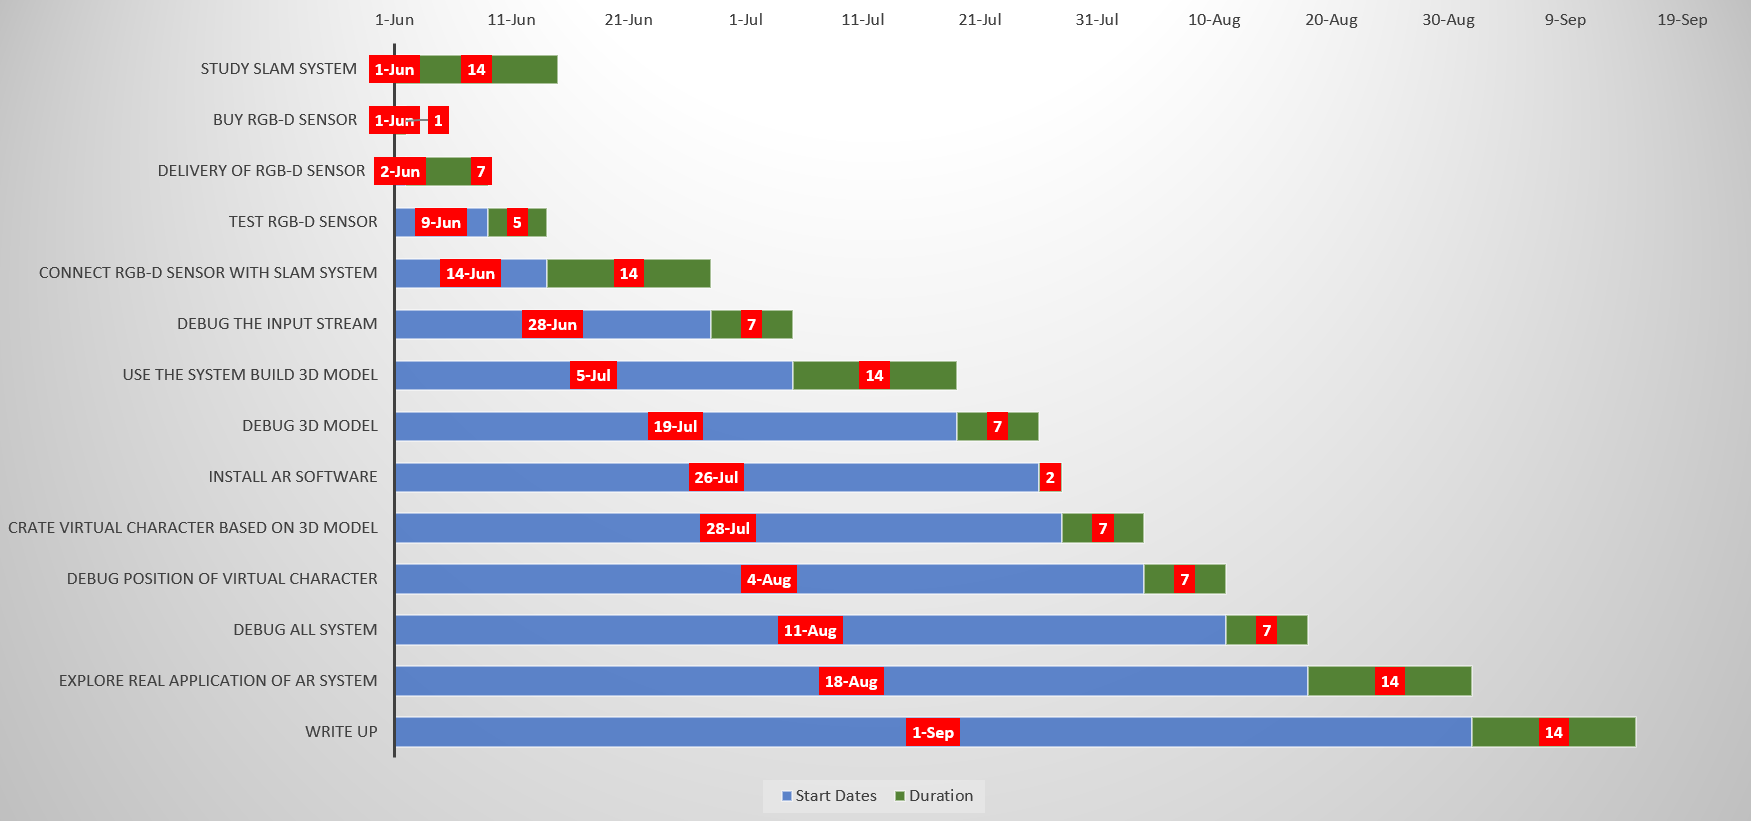
\includegraphics[height=1.1\linewidth,width=1.5\linewidth,angle=-90]{20.png}
\caption{\label{fig:frog}Timeline}
\end{figure}

\bibliographystyle{ieeetr}
\bibliography{zz}

\end{document}
